\chapter{背景介绍及方法综述}\label{chp:intro}
\section{问题简介}
随着技术进步和需求提升,我们在很多领域都面对海量的高维数据. 
数据挖掘的关键一步就是如何从高维数据中提取维度相对较低的有用信息.
在很多情况下,高维数据能通过低维的线性模型很好地近似,其中最著名的例子就是
主成分分析(Principal component analysis, PCA), 它将数据投影到其方差最大的子空间上.
从而降低维度.

然而,很多实际问题产生的高维数据来自多个混合的低维子空间.
如\autoref{fig:Union_of_sub_model} 所示, 在没有噪音的情况下,
三维数据实际分布在一个平面和两条直线上,
所以数据在本质上来自三个低维子空间.
如果想更好地降低数据维度, 就必须找到每一个子空间,
这要求我们将数据按照它们所属的子空间分割开来, 即子空间聚类.
子空间聚类的应用非常广泛,包括运动轨迹分离~\cite{costeira1998multibody},
人脸识别~\cite{basri2003lambertian},网络跳点计数~\cite{eriksson2011high},
电影评分~\cite{zhang2012guess} 以及社交图谱~\cite{chen2014clustering}等.
对应于上面所述的应用,子空间聚类能根据运动轨迹分离刚体;
判断哪些面部照片来自同一个人; 哪些网络节点属于一个子网;
给出观影兴趣相似的用户以及发现社交网络中隐含的人际关系等.
下面给出子空间聚类的定义.
\begin{figure}[tb]
  \centering
  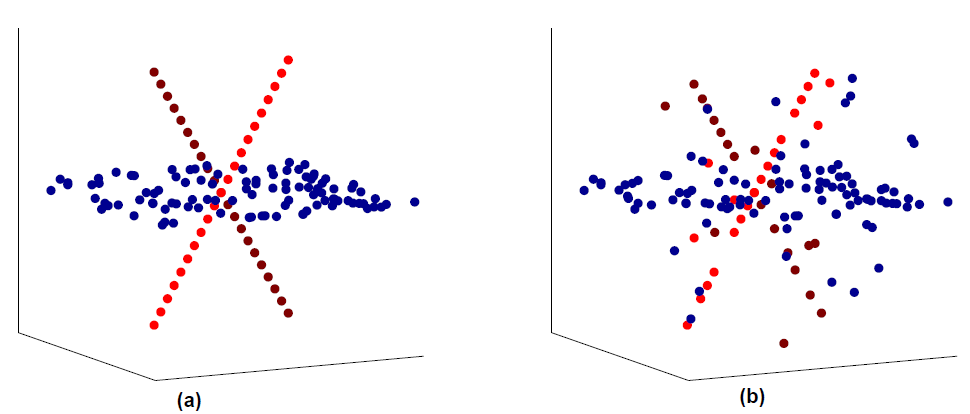
\includegraphics[width=0.8\linewidth]{Union_of_Subspace}
  \caption{采样于三个子空间的无噪音 (a) 和有噪音 (b) 数据}\label{fig:Union_of_sub_model}
\end{figure}
\begin{definition}[子空间聚类(Subspace clustering, SC)]\label{def:sc}
  有\(n\)个\(\R^d\)中的数据点\(x_i = y_i+z_i, \, i \in [n]\),
  \(y_i\)代表无噪音的理想点, \(z_i\)为噪音, \(y_i\)属于\(L\)个子空间的并
  \[\cS_1 \cup \cS_2 \cup\cdots\cup \cS_L,\]
  每个子空间\(\cS_\ell \subset \R^d\)的维度为\(d_{\ell} < d\),
  包含 \(n_{\ell}\)个数据点, 因此\(\sum_{\ell=1}^L n_\ell=n\). 
  子空间聚类是指将\(x_1, x_2, \ldots, x_n\) 分割为\(L\)类,
  使每一类对应一个子空间(注意, 下面为了表示方便, 通常把\(x_i, y_i, z_i\)
  按照列并在一起写成矩阵\(X, Y, Z\in \R^{d\times n}\)).
\end{definition}
\section{方法综述}
过去十年,子空间聚类问题引起广泛关注,人们提出了多种算法:
期望最大化(Expectation maximization)类型的局部优化算法,
比如 K-plane~\cite{bradley2000k} 和 Q-flat~\cite{tseng2000nearest};
代数方法,比如广义主成分分析(Generalized principal component analysis)~\cite{vidal2005generalized};
矩阵分解方法~\cite{costeira1995multi,costeira1998multibody}; 基于谱聚类的方法
~\cite{chen2009spectral,lauer2009spectral}; 自底向上的局部采样方法~\cite{rao2008motion,yan2006general};
以及基于自表示的方法,比如稀疏子空间聚类(Sparse subspace clustering, SSC)~\cite{elhamifar2009sparse,elhamifar2013sparse}
和低秩表示 (Low rank representation, LRR)~\cite{liu2010robust,liu2013robust}.
以上算法综述详见~\cite{vidal2010tutorial} 及其参考文献,
本文主要介绍SSC及其各种衍生算法.

\subsection{SSC和LRR}
2009年Elhamifar等首先将稀疏表示(Sparse representation)用于子空间聚类~\cite{elhamifar2009sparse}, 
提出基于自表示的SSC方法, 并在2013年加以完善~\cite{elhamifar2013sparse}, 使其成为目前公认表现最好的子空间聚类算法之一.
自表示的基本思想是: 因为数据点\(x_i\)的和另外一些点都在同一低维子空间中, 那么 
我们可以用其它点的线性组合表示\(x_i\), 即
\begin{equation}
  x_i \approx \sum_{i\neq j} [c]_j x_j, 
  \label{eq:rep}
\end{equation}
其中系数向量\(c\in \R^n, [c]_i = 0\). 
由于噪音干扰, 完全精确的表示不一定存在, 所以这里用了约等于.
如果数据点按列排成矩阵 \eqref{eq:rep} 等价于
\begin{equation}
  X \approx XC \quad \text{s.t.}\quad \diag(C) = \mathbf{0},
  \label{eq:matrix_rep}
\end{equation}
其中\(C\in \R^{n\times n}\), \(\diag(\cdot)\)是矩阵的对角线向量组成的对角阵.
利用表示矩阵\(C\)可以构造邻接矩阵\(W=(|C|+|C^T|)/2\),
这样子空间聚类问题就转化成\(n\)个点的无向图
分割问题, 我们可以谱聚类算法~\cite{ng2002spectral} 解决.

显然能否得到较好的表示系数是自表示方法成败的关键.
对于 \eqref{eq:rep} 我们希望表示系数\(c\)满足
\begin{equation}\label{eq:self_rep_1}
  [c]_j = 0, \quad  \forall j\in [n], \,y_j \notin \cS_\ell .
\end{equation}
即只用和\(x_i\)属于同一子空间的点表示\(x_i\).
这样的\(c\)必然比较稀疏(大部分位置都是零), 
于是SSC对无噪音和有噪音的数据分别求解 \eqref{eq:SSC} 和 \eqref{eq:ssc_noise}.  
\begin{gather}
  \min_{c} \; \|c\|_1\quad \text{s.t.}\quad y_i=Yc, \quad [c]_i=0 \label{eq:SSC}\\
  \min_{c} \; \|c\|_1+\frac{\lambda}{2}\left\|x_i-Xc\right\|_2^2, \quad \text{s.t.} \quad
  [c]_i = 0. \label{eq:ssc_noise}
\end{gather}
SSC利用\(\ell_1\)正则化迫使每个点只用较少的其它点表示,
这样所用点就很可能和\(x_i\)来自同一子空间.
\([c]_i = 0\)的约束是为了避免平凡解,
即每个数据仅用它自己表示自己.
Elhamifar等证明了在无噪音且子空间\(\cS_1, \cS_2, \ldots, \cS_L\)
相互独立(子空间只在原点相交)的情况下,
 \eqref{eq:SSC} 的解\(c\)满足 \eqref{eq:self_rep_1} ~\cite{elhamifar2013sparse}.
Cand\`{e}s等证明了带噪音半随机模型下, 当点和子空间分布满足一定条件时,
\(c\)有较大概率满足 \eqref{eq:self_rep_1} ~\cite{soltanolkotabi2014robust} .
把 \eqref{eq:ssc_noise} 写成矩阵的形式
\begin{equation}
  \begin{gathered}
    \min_C \; \|C\|_1+\frac{\lambda}{2}\left\|X-XC\right\|_F^2\\
    \text{s.t.} \quad \diag(C)=\mathbf{0}.
  \end{gathered}
  \label{eq:ssc_matrix}
\end{equation}
我们可以得到\autoref{alg:ssc}.  

\begin{algorithm}[tb]
  \caption{稀疏子空间聚类(Sparse subspace clustering)}
  \label{alg:ssc}
  \begin{algorithmic}
    \State {\bfseries 输入:}
    数据点组成的矩阵 \(X\in \mathbb{R}^{d\times
    n}\),类数\(L\)和正则化参数\(\lambda\)
    \State{1. } 求解 \eqref{eq:ssc_matrix},   得到最优解\(C\)
    \State{2. } 令 \(W=(|C|+|C|^T)/2\) 构造邻接图\(G\),其邻接矩阵为\(W\)
    \State{3. } 对 \(G\) 进行谱聚类 
    \State {\bfseries 输出:} 聚类结果
  \end{algorithmic}
\end{algorithm}

SSC只是单独考虑每个数据的稀疏表示, 缺少对
数据集全局结构的描述. 为反映数据集的全局结构,
2010年, Liu等提出基于低秩表示的子空间聚类方法LRR~\cite{liu2010robust} .
类似于SSC, LRR也是求解数据点的表示,
不过将\(\ell_1\)正则化换成了低秩,
\begin{equation}
  \min_{C} \; \rank(C)+\frac{\lambda}{2}\|X-XC\|_F^2. \label{eq:lrr}
\end{equation}
不过 \eqref{eq:lrr} 很难求解, 常用的办法是将\(\rank(C)\)松弛成\(\|C\|_*\),
\(\|\cdot\|_*\)是矩阵核范数,即矩阵奇异值之和.
这样 \eqref{eq:lrr} 变成一个凸优化问题. 再类似SSC,用解出的\(C\),构造
邻接矩阵\(W\), 最后谱聚类.

SSC和LRR在实际测试集上都有不错的表现.
例如在运动分割领域的Hopkins155测试集~\cite{tron2007benchmark}上,
他们都有很高的正确率~\cite{elhamifar2013sparse, liu2013robust}.
不过当类别增多时, SSC较LRR更优秀~\cite{elhamifar2013sparse}.

\subsection{其它自表示方法}
基于SSC和LRR产生了很多拓展和变形.
Wang等同时考虑低秩和稀疏性,得出了下面的优化问题~\cite{wang2013provable}
\begin{equation}\label{eq:scc_lrr}
  \begin{gathered}
    \min_{C} \; \|C\|_*+\mu \|C\|_1+\frac{\lambda}{2}\|X-XC\|^2 \\
    \text{s.t.}\quad \diag(C) = \mathbf{0}.
  \end{gathered}
\end{equation}
其中\(\mu,\lambda\)均为给定参数. 
Zhuang等在 \eqref{eq:scc_lrr} 的基础上加上系数矩阵\(C\)非负
的限制,以应用于半监督学习~\cite{zhuang2012non}.

SSC,LRR需要假定数据充足, 对样本不足的情形, Patel等
提出了隐式SSC (Latent SSC) 和隐式LRR(Latent LRR)模型~\cite{patel2015latent},
\begin{equation}
  \begin{gathered}
    \min_{P,C} \mathcal{J}_1(C)+\mathcal{J}_2(P, C, X) \\
    \text{s.t.}\quad PP^T=I, \diag(C)=\mathbf{0},
  \end{gathered}
  \label{eq:latent}
\end{equation}
其中\(\mathcal{J}_2=\lambda_1\|PX-PCX\|_F^2+\lambda_2\|X-P^TP
X\|_F^2,\)而\(\mathcal{J}_1(C)\)可以是\(\|C\|_1\)也可以是\(\|C\|_*\),
矩阵\(P\)可以看成是从原始数据空间到隐式空间线性变换,要求它的每一行
正交且模长为1. 虽然 \eqref{eq:latent} 是非凸的,但是数值实验表明
收敛到局部极小值只需要几步迭代.

为了进一步提高子空间聚类的精度, Lu使用了Trace LASSO改进SSC,
提出相关自适应子空间分割 (Correlation adaptive subspace
segmentation, CASS)~\cite{lu2013correlation}, 
对每个数据点\(x_i\)求解
\begin{equation}
  \min_{c}\, \|X\diag(c)\|_* + \frac{\lambda}{2}\|x_i - Xc\|_2^2,
  \label{eq:cass}
\end{equation}
其中\(\diag(c)\)是以\(c\)为对角线的矩阵.如果把\(X\)的每一列按照\(\ell_2\)范数
归一化,Trace LASSO具有插值性质:
\[
  \|c\|_2\le \|X\diag(c)\|_*\le \|c\|_1.
\]
左端等式在数据是完全相关时(每列方向相同或相反)达到,右端在数据是完全无关时(列之
间正交)达到,这使得Trace LASSO能自适应数据的相关性.

Cand\`{e}s等指出在原有的\(\ell_1\)正则化参数上加上
适当权重, 可以进一步提高稀疏度~\cite{candes2008enhancing}.
于是Pham等提出了加权SSC (Weighted SSC)~\cite{pham2012improved},即求解下面的优化问题
\begin{equation}
  \begin{gathered}
    \min_{C}\, \|W\odot C\|_1 + \frac{\lambda}{2}\|X-XC\|_F^2 \\
    \quad \text{s.t.}\quad \diag(C) = \mathbf{0},
  \end{gathered}
  \label{eq:wssc}
\end{equation}
其中\(W\)是某个权重矩阵,比如可以取
\[
  W_{i,j} = \left( \exp\left\{ -\frac{\|x_i-x_j\|_2}{\mu}
\right\} \right)^{-1},
\]
其中\(\mu\)是给定参数.由于实际应用中空间距离近的点是同类的概率较大,
上面的权重矩阵可以使自表示时更倾向于用附近的点,从而提高准确率.

如果SSC或者LRR产生的邻接矩阵是严格块对角的, 那么谱聚类的效果
很可能较好,所以Feng等提出块对角稀疏子空间聚类
(Block-diagonal sparse subspace clustering, BD-SSC)模型~\cite{feng2014robust}.
在优化 \eqref{eq:ssc_noise} 和 \eqref{eq:lrr} 时, BD-SSC加上了\(C \in \cK\) 的限制,其中
\[
  \cK = \left\{ \rank(L_W)=n-L, W=\half\left( |C|+|C^T| \right) \right\},
\]
\(L\)是子空间类数,\(L_W=\diag(W)-W\).
在寻找表示矩阵\(C\)时, BD-SSC预先要求其有比较好的可分性, 从而提高谱聚类正确率. 
不过如此一来优化问题高度非凸, 虽然可以用交替方向投影方法求解, 但是结果比较依赖初始值选取.

Yuan等首先引入组稀疏范数, 提出了稀疏生成子空间聚类
(Sparse additive subspace clustering, SASC)~\cite{yuan2014sparse}.
其想法是: 虽然同类的数据点理论上在一个线性子空间中,
但由于噪音干扰可能失去了线性性, 因此直接做线性回归无法取得好的效果,
如果我们用一族变换\(\left\{T_1, T_2, \cdots, T_m\right\}\)作用到每个点\(x_i\)上,
可以生成\(m\)个新的数据点\(\left\{ T_1 x_i, T_2 x_i,\cdots,
T_m x_i \right\}\),其中很可能包含比\(x_i\)更接近无噪音的点. 
我们把每个原始的数据点\(x_i\)相对于\(n\times m\)个新生成的
数据点做回归,由于新数据天然具有组别(同一点生成的自然是一组),
令代表组别信息的指标集族
\begin{equation*}
  \Omega:= \left\{ \{1,\ldots, m\}, \{m+1, \ldots, 2m\}, \ldots, \{(n-1)m+1,
  \ldots, nm\}\right\}.
\end{equation*}
对每个\(x_i\)求解
\begin{equation}
  \begin{gathered}
    \min_{c}\, \|c\|_{\Omega, 1}+\frac{\lambda}{2}\|x_i-\left[ 
      T_1 x_1, \cdots, T_m x_1,\cdots, T_1 x_n, \cdots, T_m x_n
    \right] c\|_2^2 \\
    \text{s.t.} \quad [c]_j = 0,\,\, (i-1)m < j \le i\cdot m,
  \end{gathered}
  \label{eq:sasc}
\end{equation}
其中\(\|c\|_{\Omega, 1}\)范数是将向量的分量\(m\)个一组,每组的\(\ell_2\)范数加和.
SASC在变换选取适当时,有很好的表现,但是变换选取的不确定性是其重要缺陷.
